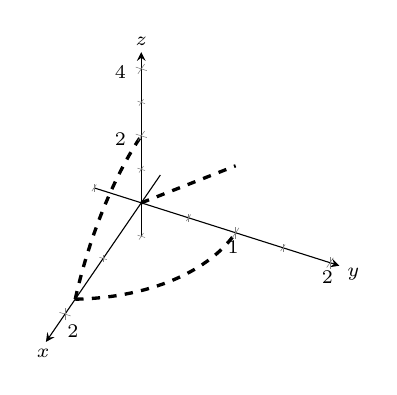
\begin{tikzpicture}[>=stealth]
\begin{axis}%
[width=175pt,height=200pt,
tick label style={font=\scriptsize},axis on top,
			axis lines=center,
			view={115}{45},
			name=myplot,
			%xtick={1,2,3,4},
			%ytick={1,2,3,4,5,6},
			%ztick=\empty,
			%extra x ticks={1},
			minor x tick num=1,
			minor y tick num=1,
			minor z tick num=1,
			%extra x tick labels={$a$},
			%extra y ticks={1},
			%extra y tick labels={$a$},
			%extra z ticks={1},
			%extra z tick labels={$h$},
			ymin=-.5,ymax=2.1,
			xmin=-.5,xmax=2.5,
			zmin=-1, zmax=4.5,
			every axis x label/.style={at={(axis cs:\pgfkeysvalueof{/pgfplots/xmax},0,0)},xshift=-1pt,yshift=-4pt},
				xlabel={\scriptsize $x$},
			every axis y label/.style={at={(axis cs:0,\pgfkeysvalueof{/pgfplots/ymax},0)},xshift=5pt,yshift=-3pt},
				ylabel={\scriptsize $y$},
				every axis z label/.style={at={(axis cs:0,0,\pgfkeysvalueof{/pgfplots/zmax})},xshift=0pt,yshift=4pt},
				zlabel={\scriptsize $z$}
			]



%\addplot3[domain=0:360,,y domain=0:4,%surf,%fill=white,
%%colormap={mp2}{\colormapplaneone},opacity=.6,faceted color=black!40,
%samples=30,smooth,,samples y=0,dashed,very thick,{\colorone}] ({cos(x)+2},{sin(x)+2},{0});

%\addplot3[domain=0:2,,y domain=0:1.5,surf,%fill=white,
%colormap={mp2}{\colormapplaneone},opacity=.6,faceted color=black!40,samples=15,samples y=15,very thin,z buffer=sort] {3-x^2-y^2};
%
%\addplot3[domain=0:2,,y domain=0:2,surf,%fill=white,
%colormap={mp2}{\colormaptwo},opacity=.6,faceted color=black!40,samples=2,samples y=2,very thin,z buffer=sort] {2*y};


%\addplot3[domain=30:90,,y domain=0:4,%surf,%fill=white,
%%colormap={mp2}{\colormapplaneone},opacity=.6,faceted color=black!40,
%samples=30,smooth,,samples y=0,very thick,{\colorone}] ({2*cos(x)},{2*sin(x)-1},{3-(2*cos(x))^2-(2*sin(x)-1)^2});

\addplot3[domain=30:90,,y domain=0:4,%surf,%fill=white,
%colormap={mp2}{\colormapplaneone},opacity=.6,faceted color=black!40,
samples=30,smooth,,samples y=0,very thick,{\colorone},dashed] ({2*cos(x)},{2*sin(x)-1},{0});

\addplot3[domain=30:90,,y domain=0:4,%surf,%fill=white,
%colormap={mp2}{\colormapplaneone},opacity=.6,faceted color=black!40,
samples=30,smooth,,samples y=0,very thick,{\colorone},dashed] ({2*cos(x)},{0},{(4*sin(x)-2)});

\addplot3[domain=0:1,,y domain=0:4,%surf,%fill=white,
%colormap={mp2}{\colormapplaneone},opacity=.6,faceted color=black!40,
samples=30,smooth,,samples y=0,very thick,{\colorone},dashed] ({0},{x},{2*x});

%\draw [{\colorone}, very thick] (axis cs:0,0,0) -- (axis cs:0,0,2)
																		%(axis cs:0,0,0) -- (axis cs:3,0,0)
																		%(axis cs:0,0,0) -- (axis cs:0,6,0);
		

%\draw [{\coloronefill},thin,fill={\coloronefill},opacity=.6] (axis cs: 3,0,0) -- (axis cs: 0,6,0) -- (axis cs: 0,0,2)--cycle;





\end{axis}


\end{tikzpicture}












